\documentclass{ximera}  


\input{../preamble.tex}



 
\title{Electrostatic Potential} 
\author{Milica Markovic} 
\outcome{Electrostatic potential.}
\begin{document}  
\begin{abstract}  

\end{abstract}  
\maketitle    






\section{Electrostatic Potential Energy}


When charges are pushed around in an electric field, the energy is not lost. Electrical forces are conservative. 


How much energy do we have to bring into the system to bring two far-away positive charges at a distance r?

To answer that question, we can look at Figure \ref{Potential1}. Bringing the first charge to a certain position in space would require no work since there are no other charged particles around, no electric field, and therefore no force.  To bring the second charge at a distance r from the first charge, we need to overcome the repulsive force between the charges. How much work does this take? 
The work that we need to do to bring charges together is equal to the work that the first charge has to do to repel the second charge. The only difference is that we have to move the charges closer together, from infinity to some distance r, and the repulsive force does the work (pushes the charge $q_2$ away) from the distance r to infinity.



\begin{figure}[htbp]
\begin{center}
\includegraphics[scale=0.5]{../jpg/Two_Static_Charges_Potential.jpg}
\end{center}
\caption{Moving the charge $q_2$ with force $\vec{F}_{us}$ against the electrostatic force $\vec{F}_e$ due to charge $q_1$ to find the electrostatic potential energy}\label{Potential1}
\end{figure}


\begin{eqnarray}
W_{us}=W{e} \\
W_{us}= \int_{\infty}^{r} \vec{F}_{us} \cdot \vec{dr} \\
W_{e}=  \int_{r}^{\infty} \vec{F}_{e} \cdot \vec{dr} 
\end{eqnarray}

The electric force is $\vec{F}_e=\frac{q_1 q_2}{4 \pi \epsilon_o r^2} \vec{r}$, so we can calculate the total work necessary to bring the two charges at distance r.

\begin{eqnarray}
W_{us}= \int_{r}^{\infty} \vec{F}_{e} \cdot \vec{dr} \\
W_{us}= \int_{r}^{\infty} \frac{q_1 q_2}{4 \pi \epsilon_o r^2} \vec{r} \vec{dr}
\end{eqnarray}

Since the charge is moved in the direction of the force, we can drop vectors and calculate the work we have to do.

\begin{eqnarray}
W_{us}= \frac{q_1 q_2}{4 \pi \epsilon_o} \int_{r}^{\infty} \frac{dr}{r^2} \\
W_{us}=  \frac{q_1 q_2}{4 \pi \epsilon_o} (-\frac{1}{r}\Big|_{r}^{\infty})
W_{us}=  \frac{q_1 q_2}{4 \pi \epsilon_o r} \label{WorkPoinCharge}
\end{eqnarray}

This work is the same no matter what path we take to move charge $q_2$ from infinity to a distance r from charge $q_1$, see Figure \ref{PotentialWork}. It depends only on the initial and end position of the charge.





\begin{figure}[htbp]
\begin{center}
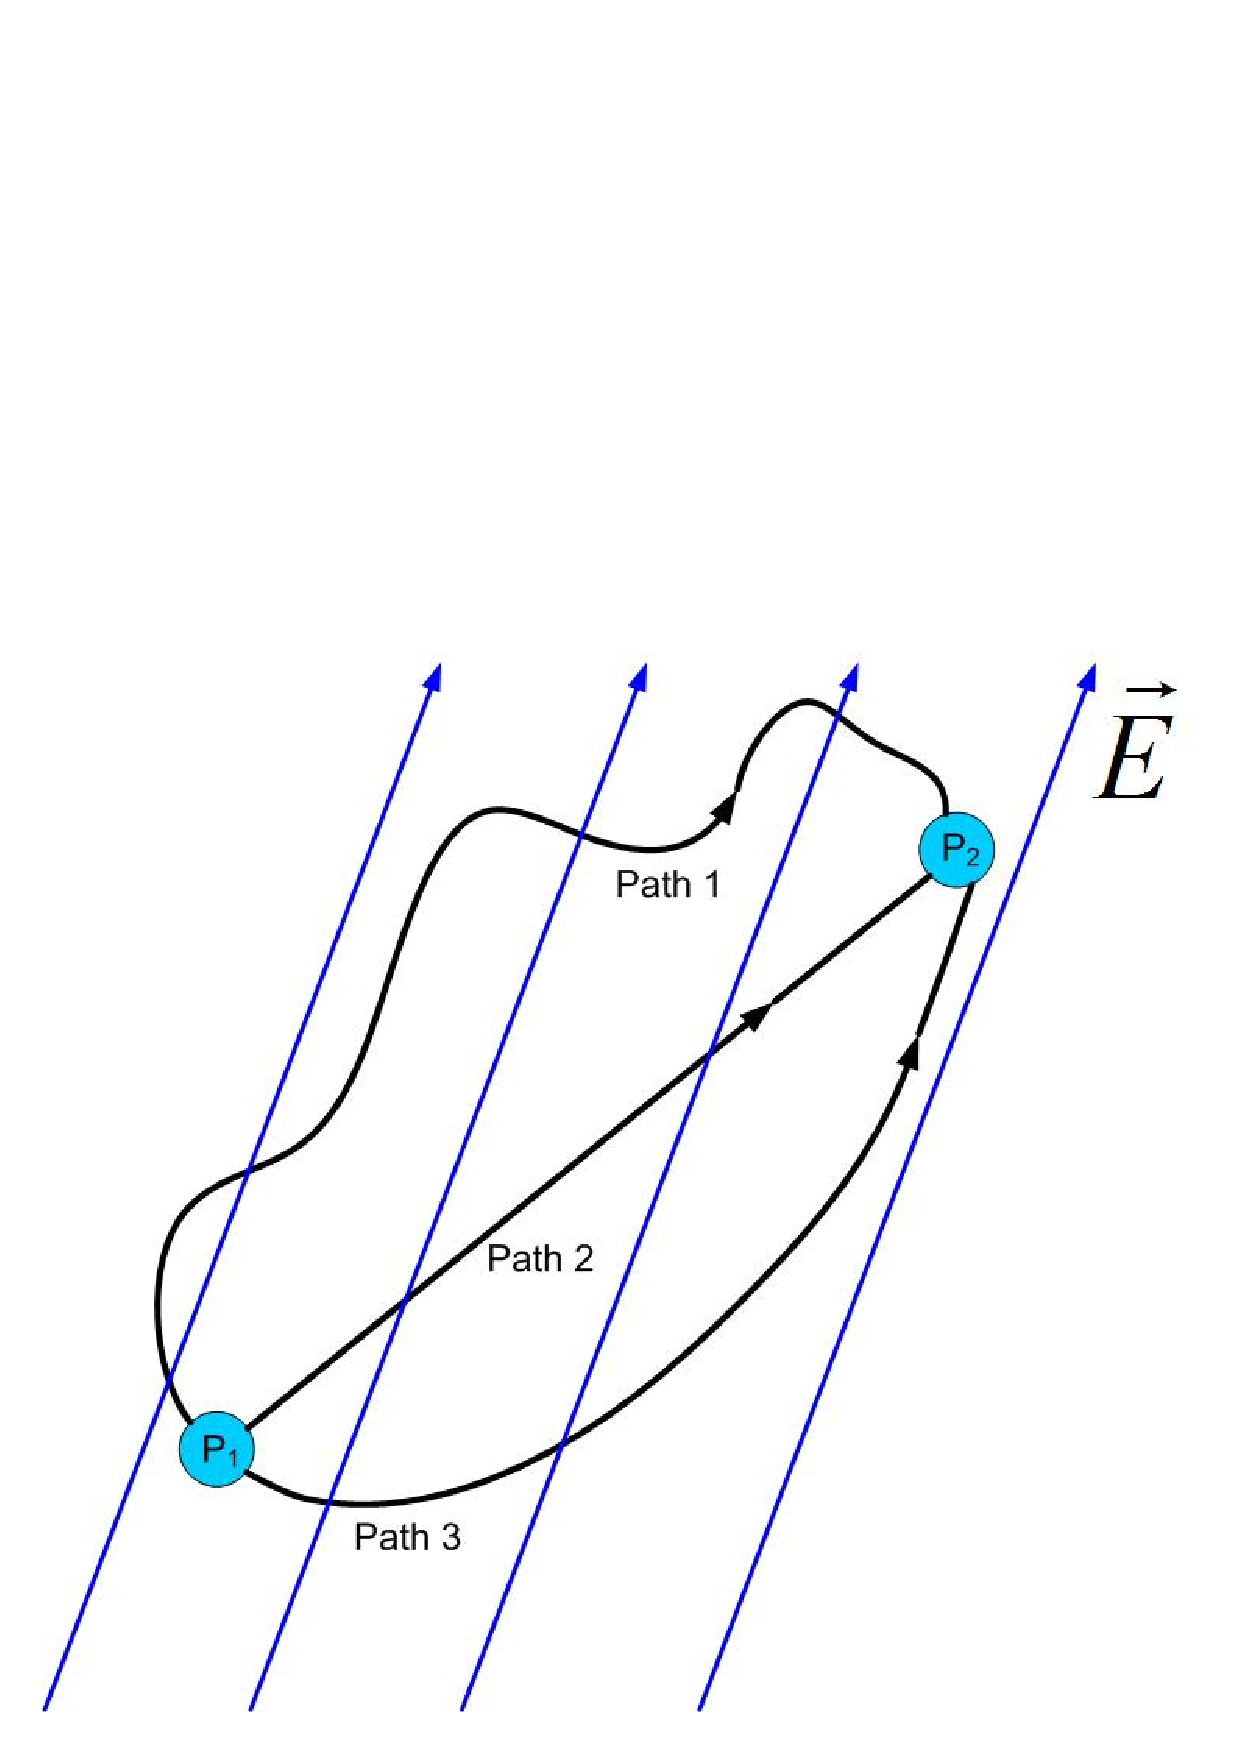
\includegraphics[scale=0.5]{../jpg/workindependentofpath.jpg}
\end{center} 
\caption{Potential is not dependent on the specific path.}\label{PotentialWork}
\end{figure}







\section{Definition of Potential and Voltage}


The work needed to move the two charges closer together depends on both charges $q_1$ and $q2$, just like the electrostatic force depends on both charges. It would be easier to define another variable that will separate the cause, charge $q_1$, and the effect, the work that we have to do to move charge $q_2$. This variable is Electric Potential. Electric potential is defined as the work we need to do to move the charge divided by the amount of charge $q_2$.

\begin{eqnarray}
V=\frac{W_{us}}{q_2} \\
V=\frac{q_1}{4 \pi \epsilon_o r} \label{Potential2}
\end{eqnarray}

Observe that in Equation \ref{Potential2} the potential is a function of the "source" charge $q_1$. We again separated the source and the effect, but this time of the potential energy. The source is a charge $q_1$ that produces potential V. If we now want to see what is the potential energy or work that we need to do to move another charge, we don't have to know which charge produced it. We only need to know the potential in an area, from which we can find the potential energy change of charge $q_2$. 

We can find potential energy and potential of any number of charges using the above expression and the principle of superposition. 


\begin{question}  
The difference in electric potential is most closely associated with 
\begin{multipleChoice}  
\choice[correct]{Work per unit charge}  
\choice{Number of electrons in an atom}  
\choice{Mechanical force on a charge}  
\end{multipleChoice}  
\end{question}

\section{The general relationship between the electric field and potential}

In the first section, we defined the work necessary to bring two charges togeter at a distance r as 

\begin{eqnarray}
W_{us}=  \int_{r}^{\infty} \vec{F}_{e} \cdot \vec{dr}\label{eqn:definitionWork} 
\end{eqnarray}

Electric force can be expressed in terms of electric field as

\begin{equation}
\vec{F}=q \vec{F}
\end{equation}

If we substitute the electric force from the above equation into Equation \ref{eqn:definitionWork}, we get 

\begin{eqnarray}
V_R=  \int_{r}^{\infty} q \vec{E} \cdot \vec{dr}
\end{eqnarray}

The potential of a point R with respect to infinity is then defined as 

\begin{eqnarray}
V_R=\frac{W_{e}}{q}=\int_{r}^{\infty}  \vec{E} \cdot \vec{dr}
\end{eqnarray}


The potential at a point due to a unit positive charge is found to be V.  If the distance between the charge and the point is tripled, the potential becomes 

\begin{question}  
The potential at a point due to a unit positive charge is  V.  If the distance between the charge and the point is doubled, the potential becomes 
\begin{multipleChoice}  
\choice{$V^2$}  
\choice{$2V$}  
\choice[correct]{$V/2$}
\choice{need more information}  
\end{multipleChoice}  
\end{question}



\section{Voltage - the potential difference}

The potential difference between two points is  defined as $V_{AB}=V_A-V_B$. We defined the potential at a point in the equation above as


\begin{eqnarray}
V_A=\int_{A}^{\infty}  \vec{E} \cdot \vec{dr} \\
V_B=\int_{B}^{\infty}  \vec{E} \cdot \vec{dr} 
\end{eqnarray}

The potential difference, or voltage is then defined as


\begin{eqnarray}
\Delta V = V_A - V_B =\int_{A}^{\infty}  \vec{E} \cdot \vec{dr} -\int_{B}^{\infty}  \vec{E} \cdot \vec{dr}  \\
\Delta V = \int_{A}^{\infty}  \vec{E} \cdot \vec{dr} +\int_{\infty}^{B}  \vec{E} \cdot \vec{dr} \\
\Delta V = \int_{A}^{B} \vec{E} \cdot \vec{dr} 
\end{eqnarray}

Demonstration of potential difference in radial electric field of a VanDenGraaf generator by Prof. Emeritus at MIT, Walter Lewin.
\begin{center}  
\youtube{cYOBSzh2SLE}  
\end{center}


Now you can enjoy shocking John Travoltage in this PhET simulation. 



\begin{center}  
\geogebra{zm6qzDwt}{1000}{800}  
\end{center} 

\section{Electric field calculation from potential difference}

From the equation above, if we look at the potenital of two points that are very close on the x-axis, $V_A$, and $V_B=V_A+dV$, the voltage is equal to $V_A-V_B=V_A-(V_A+dV)=-dV=-E_x dx$. Therefore the electric field in the x-direction is 

\begin{equation}
\vec{E_x}=-\frac{\partial V}{\partial x} 
\end{equation}

The above equations states that the field is proportional to the change of potential over distance. The larger the change of potential over distance, the stronger the field.

To find the electric field in 3 dimensions, we use the gradient function, which represents a 3-dimensional derivative.

\begin{equation}
\vec{E}=-\grad V = -(\frac{\partial V}{\partial x}\vec{x}+\frac{\partial V}{\partial y}\vec{y}+\frac{\partial V}{\partial z}\vec{z})
\end{equation}


\begin{example}
Figure \ref{fig:gradient} shows an electric field, and equipotential lines in an x-y plane. Equipotential lines are the lines of the same potential. We can observe that the electric field is always normal to the equipotential lines. The difference in potential between two points is $dV=\vec{E} \vec{dr}$. The lines, or surfaces, normal to the electric field vector are always equipotential surfaces, as the angle between the electric field vector and a perpendicular vector is $90^0$, and the dot product between them is zero. In other words, the work that we have to do to move the charge in the direction perpendicular to the electric force is zero.

\begin{figure}[htbp]
\begin{center}
\includegraphics[scale=0.4]{../jpg/gradient.jpg}
\end{center} 
\caption{Electric field and equipotential lines.}\label{fig:gradient}
\end{figure}

\end{example}




\begin{example}
Two charges, a positive and a negative one are placed on x-y plane. The potential around the charges is shown as a red surface. Observe the simulation below. 

\begin{enumerate}
\item Where is the potential positive, and where is it negative? 
\item What is the direction of the electric field? 
\item If we place a positive point charge closer to the positive charge Q1, which way will it go?
\item What if we have a negative charge?
\end{enumerate}
Now click on the 2D view.
\begin{enumerate}
\item Where is the field the strongest? 
\item Can you tell the direction of the field from equipotential lines?
\end{enumerate}

\begin{center}  
\geogebra{tmkauhfc}{1000}{800}  
\end{center} 

\end{example}


\begin{problem}
Rougly adjust the direction and length of the vectors shown in the graph below. When done, click on "Grade Update " to check your answer.

\begin{center}  
\geogebra{dqvffmrh}{1000}{800}  
\end{center} 

\end{problem}



\end{document} 

